\section{GUI - Package Structure}
\begin{figure}[!ht]
\begin{center}
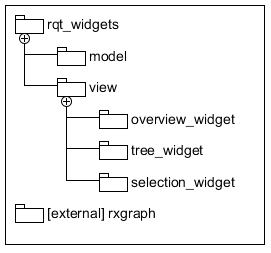
\includegraphics[scale=1.0]{./bilder/package_structure_gui.png}
\caption{The package structure of the GUI}
\label{The package structure of the GUI}
\end{center}
\end{figure}

\mbox{}

\newpage


\section{GUI - Model}
\begin{figure}[!ht]
\begin{center}
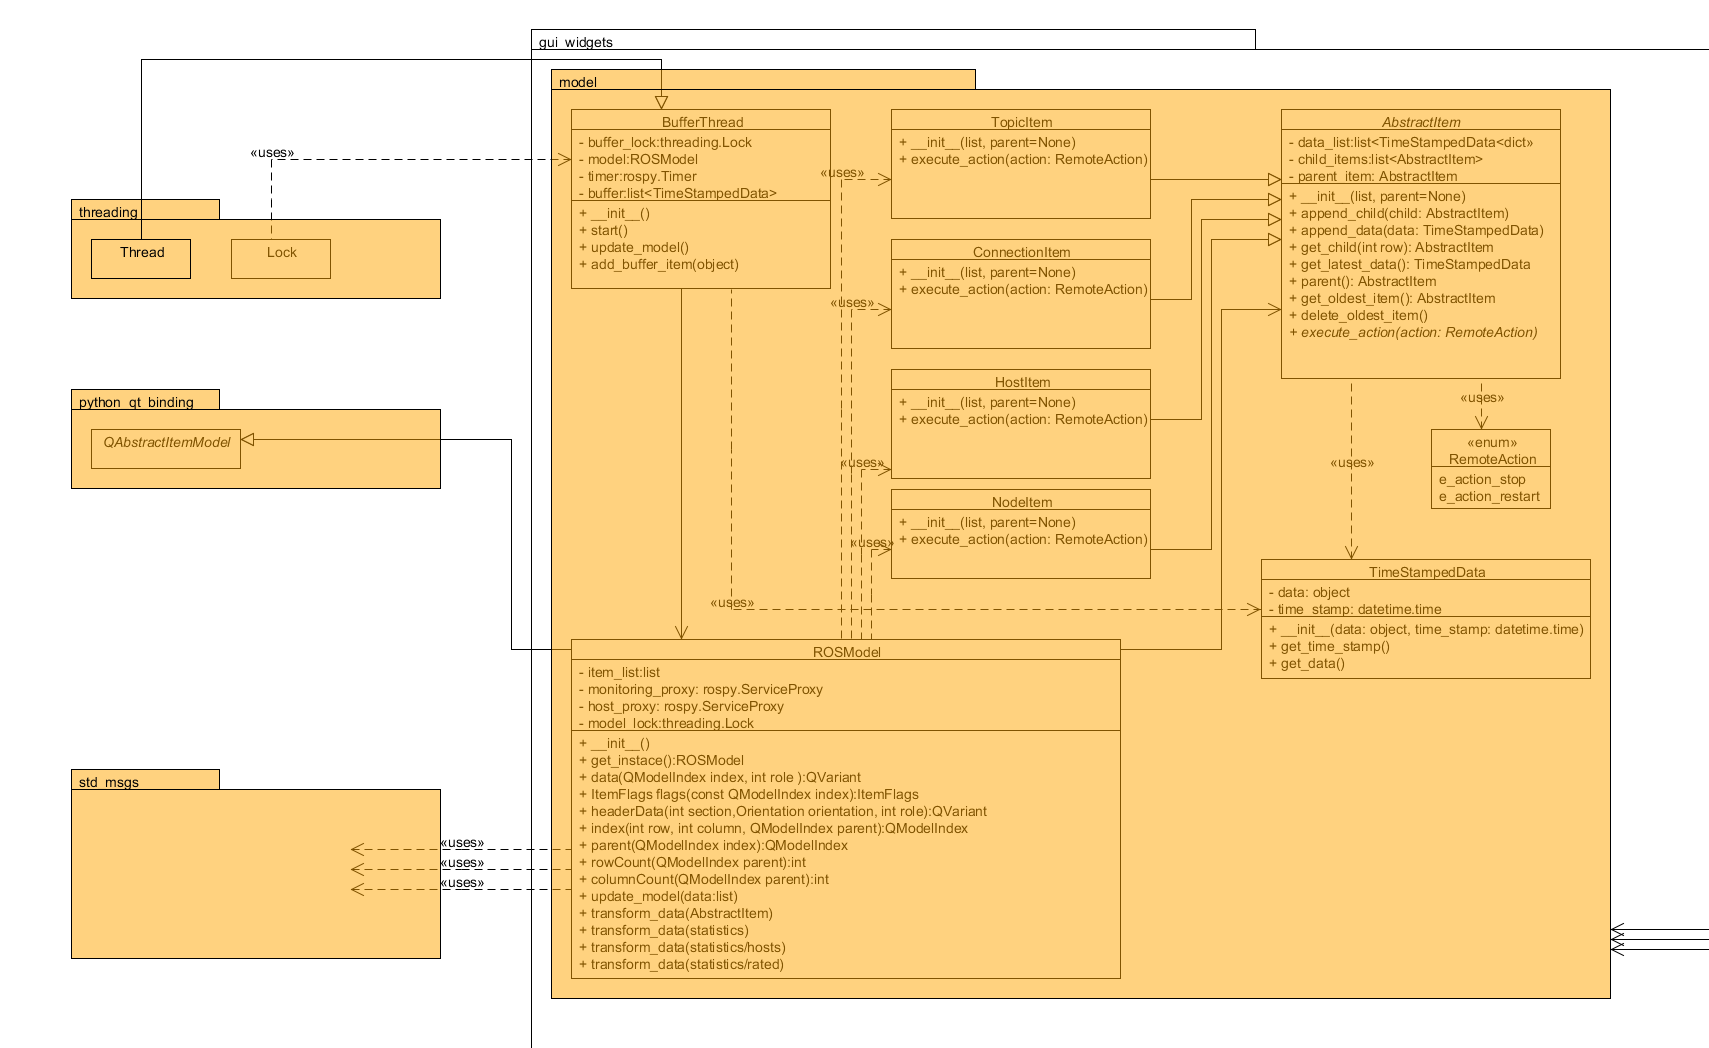
\includegraphics[width=1.0\linewidth]{./bilder/model.png}
\caption{The model class diagram}
\end{center}
\end{figure}

\subsection{BufferThread}
This thread should buffer the incoming data and regulary update the model and
hence also the model.
\subsection{ROSModel}
Represents the data as a QtModel. This enables automated updates of the View.
\subsection{ItemInterface}
Provides a unified interface to access the items of a model.
\subsection{HostItem}
A HostItem represents a host with all its data.
\subsection{NodeItem}
 A NodeItem represents a node with all of its data. It also has a interface to start/stop/restart nodes.


\section{GUI - View}
\begin{figure}[!ht]
\begin{center}
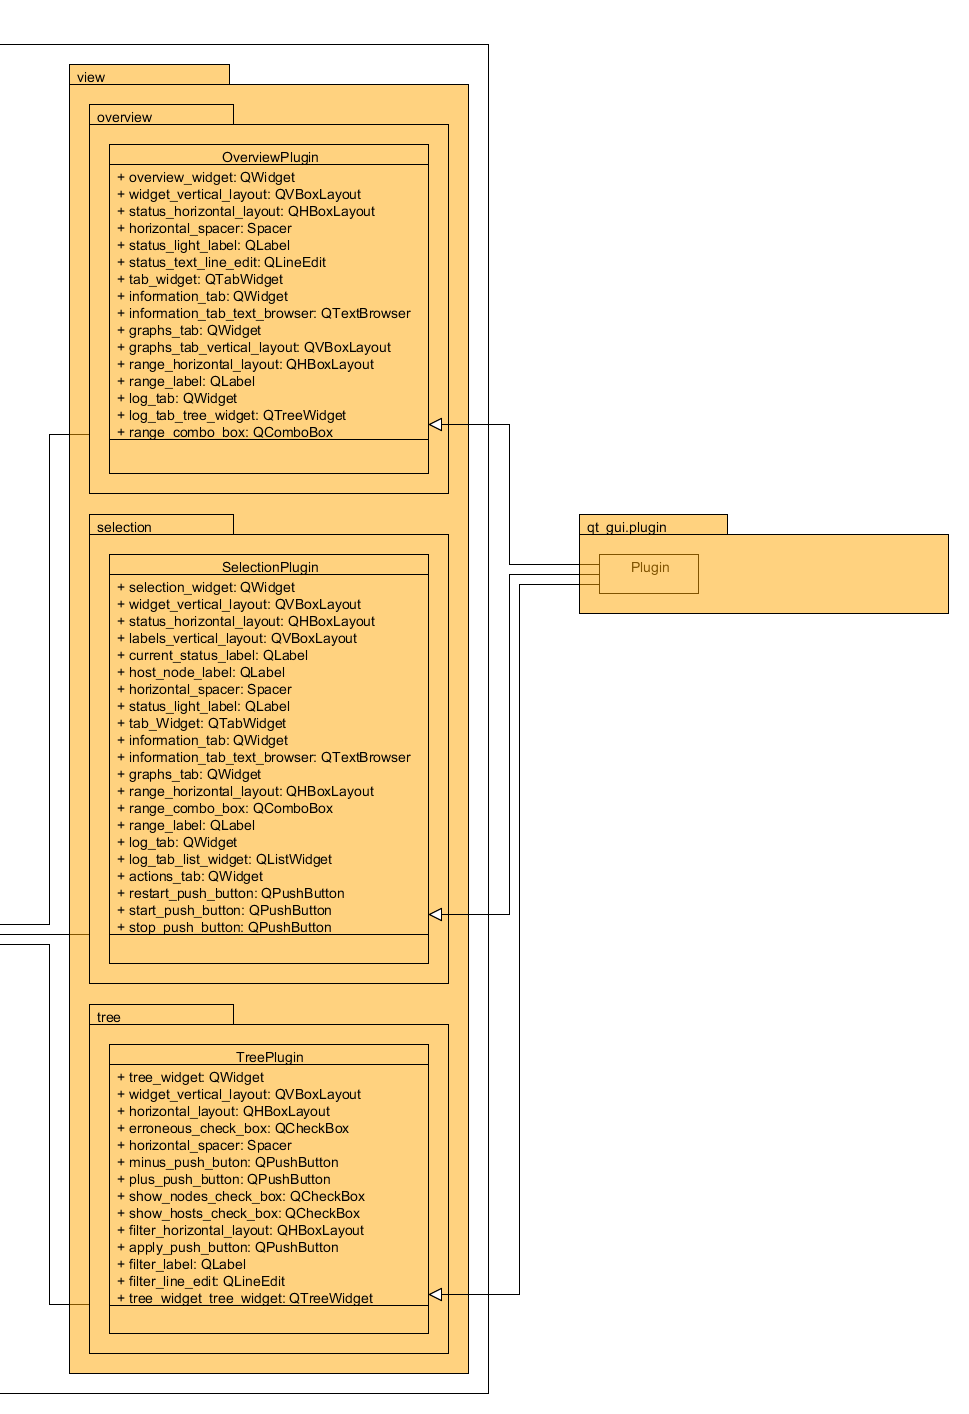
\includegraphics[width=\linewidth]{./bilder/view.png}
\caption{The view class diagram}
\end{center}
\end{figure}

\subsection{OverviewPlugin}
The class OverviewPlugin is the core of the graphical user interface, which
contains most of the relevant information in a small and fancy area.
\subsubsection{Attributes}
\begin{itemize}
  \item public overview\_widget: QWidget\\
  the object wich holds the widget
  \item public status\_light\_label: QLabel\\
  shows the actual status of the host/node
  \item public tab\_widget: QTabWidget\\
  the object wich holds the different tabs of the widget
  \item public information\_tab: QWidget\\
  a tab wich gives general information about the network 
  \item public graphs\_tab: QWidget\\
  shows the actual Network- and CPU-Load
  \item public range\_combo\_box: QComboBox\\
  makes it possible to set the range of the graphs
  \item public log\_tab: QWidget\\
  shows actual errors and warnings
  \item public log\_tab\_tree\_widget: QTreeWidget\\
  the structure of the log-messages  
\end{itemize}

\subsection{SelectionPlugin}
A class which shows detailed information in a Tree-Layout about the currently
selected host or node.
\subsubsection{Attributes}
\begin{itemize}
  \item public selection\_widget: QWidget\\
  the object wich holds the widget
  \item public host\_node\_label: QLabel\\
  shows the name of the actual selected host or node
  \item public status\_light\_label: QLabel\\
  shows the status of the host or node
  \item public tab\_widget: QTabWidget\\
  the object wich holds the different tabs of the widget
  \item public information\_tab: QWidget\\
  a tab wich gives general information about host or node 
  \item public graphs\_tab: QWidget\\
  shows the actual Network- and CPU-Load
  \item public range\_combo\_box: QComboBox\\
  makes it possible to set the range of the graphs
  \item public log\_tab: QWidget\\
  shows actual errors and warnings
  \item public actions\_tab: QWidget\\
  includes buttons to start/restart/stop nodes
  
\end{itemize}

\subsection{TreePlugin}
TreePlugin is very simply and shows only the actual active hosts
and nodes.
\subsubsection{Attributes}
\begin{itemize}
  \item public tree\_widget: QWidget\\
  the object wich holds the widget
  \item public erroneous\_check\_box: QCheckBox\\
  displays only erroneous hosts and nodes
  \item public show\_node\_check\_box: QCheckBox\\
  displays nodes
  \item public show\_host\_check\_box: QCheckBox\\
  ..hosts
  \item public minus\_push\_button: QPushButton\\
  makes it possible to zoom out
  \item public plus\_push\_button: QPushButton\\
  ..zoom in
  \item public filter\_line\_edit: QLineEdit\\
  a textfield where you can filter the output
\end{itemize}

